\documentclass[aps,prl,twocolumn,superscriptaddress,nofootinbib]{revtex4-1}

% the percent sign gives comments in Latex
% top line indicates this is for Physical Review, standard journal format,
% suitable for electronic submission of articles

% the line above is necessary to start any latex document.
% this is one variation that should work for most things.
% if you want double spaceing, use the following:
%
%\documentclass[prd,preprint,letterpaper]{revtex4}
%
% the "preprint" designation will make a wider line
% spacing, good for markup.
\usepackage{graphicx}  % this is the up-to-date package for all figures
\usepackage{amssymb}   % for math
\usepackage{verbatim}  % for the comment environment
\usepackage{color}
\usepackage{gensymb}
\usepackage{amsmath}

\usepackage[section]{placeins}

\usepackage{wrapfig}
\usepackage{hyperref}
\usepackage{titlesec}
\usepackage{amssymb}   % for math
\usepackage{verbatim}  % for the comment environment
\usepackage{color}
\usepackage[nodisplayskipstretch]{setspace}
\usepackage{amsmath}
\usepackage{blindtext}
%\usepackage[pdftex]{graphicx}
\usepackage[outdir=./]{epstopdf}
\usepackage[space]{grffile}
\usepackage{epsfig}
\usepackage[separate-uncertainty=true]{siunitx}
\usepackage{tikz}
\usepackage{pgfgantt}
\usepackage[english]{babel}
\usepackage[utf8]{inputenc}

\titlespacing*{\section}
{0pt}{1\baselineskip}{.5\baselineskip}

\titlespacing*{\subsection}
{0pt}{1\baselineskip}{.3\baselineskip}

\setlength{\textfloatsep}{1\baselineskip plus 0.2\baselineskip minus 0.5\baselineskip}

\usepackage{footnote}

\bibliographystyle{apsrev}


% these are some custom control of the page size and margins
% \topmargin= 0.2in  % these 1st two may be needed for some computers
% \textheight=8.75in
%\textwidth=6.5in
%\oddsidemargin=0cm
%\evensidemargin=0cm

% this is where the actual document itself (rather than control statements) begins:

\begin{document}

% use a style that gives automatic headings
%\pagestyle{headings}



% the \title{} command generates a title.

% the \\ below is used to FORCE a line break in the middle of the sentence--
% otherwise latex computes it for you

\title{X-ray Diffraction}


\author{\textbf{Bryan Yamashiro}}
\author{Brandon Agtarap}
\author{Corey Mutnik}
\author{Daichi Hiramatsu}
%\author{Christina Nelson}

\affiliation{Department of Physics \& Astronomy, \\
University of Hawaii at Manoa,\\
2505 Correa Rd, Honolulu, HI, 96822, USA}





	      % \section is used to start a new one with a heading
\begin{abstract}

This study aimed to utilize an x-ray apparatus to determine the crystal structures and lattice constants of sodium chloride and lithium fluoride\,\cite{1}. The sodium chloride lattice constants of the K$_\beta$ peaks for n=1 and n=2 and the K$_\alpha$ peaks for n=1 and n=2 were (596.3$\pm$10.8)\,pm, (574.3$\pm$4.5)\,pm, (595.8$\pm$9.7)\,pm, and (574.0$\pm$3.9)\,pm, respectively. The correlating errors compared to the actual value of 564.0\,pm, in order, were 3.0$\sigma$, 2.3$\sigma$, 3.3$\sigma$, and 1.0$\sigma$. The lithium fluoride lattice constants of the K$_\beta$ peaks for n=1 and n=2 and the K$_\alpha$ peak for n=1 were (407.0$\pm$4.9)\,pm, (404.4$\pm$1.9)\,pm, (411.6$\pm$4.4)\,pm, respectively. The correlating errors compared to the actual value of 403.0\,pm, in order, were 0.8$\sigma$, 0.7$\sigma$, and 1.9$\sigma$. 
%The sigma deviations of LiF ranged between 0.77$\sigma$ to 1.94$\sigma$. The low sigma results showed that the lithium fluoride quite accurately determined the lattice constant. Conversely, the sodium chloride sigma errors ranged between 2.27$\sigma$ to 3.28$\sigma$, which showed more deviation, but was still acceptable.



\end{abstract}

\maketitle    % this line is necessary to tell latex you are done with all
	      % of the stuff associated with the title, and now it can go
              % ahead and generate the title portion


\section{Background and Significance}
X-ray diffraction occurs when x-rays deflect off of structures within a crystal. The deflection maxima carry information about the arrangement of the crystalline structure in question. At 22 years old, William Bragg used x-rays to determine spacing of atoms within solid crystals. The discovery led to the practice of x-ray crystallography, and in 1953 the method was used to reveal the structure of DNA\,\cite{2}. X-ray diffraction allows for researchers to study the micro-structures of crystals with precision.

 % the ~\cite{ } is how you link a reference in the text. The references
 % themselves are at the end.

% one or more lines of space between paragraphs determines them

\section{Apparatus}


The study utilized an x-ray emitting apparatus seen in figure\,\ref{appar}. The x-ray source was supplied with a high voltage source\,(HV 1), outputting 20\,kV. The electronics in figure\,\ref{scheme} included a second high voltage source\,(HV 2), outputting 0.384\,kV. HV 2 was supplied to the Geiger-Muller\,(GM) counter. Output of the GM counter is amplified by a preamplifier and fed to a scaler. A terminated oscilloscope was also connected to the scaler to determine potential noise pulses. Apparatus components, including the target sample, between the x-ray apparatus and GM counter in figure\,\ref{scheme} are illustrated in figure\,\ref{appar}.

\begin{figure}[b]
    \begin{center}
    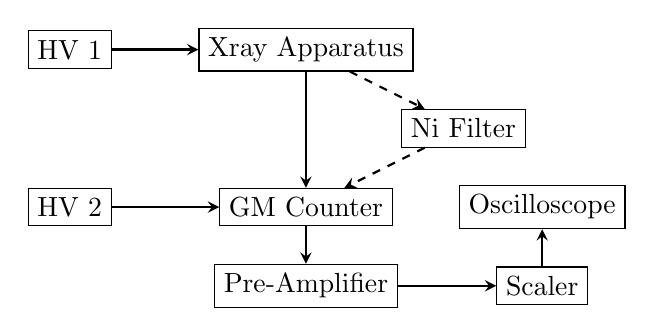
\begin{tikzpicture}[node distance=.3cm]
      %http://www.texample.net/tikz/examples/feature/arrows/
      \usetikzlibrary{shapes.geometric, arrows} 
      \tikzstyle{startstop} = [rectangle, rounded corners, minimum width=.2cm, minimum height=.2cm,text centered, draw=black]
      \tikzstyle{rect} = [rectangle, minimum width=.2cm, minimum height=.2cm, text centered, draw=black]%, fill=orange!30]
      \tikzstyle{parallelogram} = [diamond, minimum width=.2cm, minimum height=.2cm, text centered,draw=black]
      \tikzstyle{arrow} = [thick,->,>=stealth]
      \node (Zname) at (-6,5) [rect] {HV 1};
      \node (Sname) at (-3,5) [rect] {Xray Apparatus};
      \node (Aname) at (-6,3) [rect] {HV 2};
      \node (Bname) at (-3,3) [rect] {GM Counter};
        \node (Kname) at (-1,4) [rect] {Ni Filter};
      \node (Cname) at (-3,2) [rect] {Pre-Amplifier};
      \node (Dname) at (0,2) [rect] {Scaler};
      \node (Ename) at (0,3) [rect] {Oscilloscope};
      %\node (Fname) at (-3,0) [rect] {Scaler};
      %\node (Gname) at (0,0) [rect] {Counter};
      %\node (Hname) at (-3,-1) [rect] {TAC};
      %\node (Iname) at (-3,-2) [rect] {MCA};
      %\node (Jname) at (-3,-3) [rect] {Computer};

      \draw [arrow] (Aname) -- (Bname);
      %\draw [dashed,arrow] (Bname) -- (Cname);
        \draw[dashed,arrow] (Sname) -- (Kname);
        \draw[dashed,arrow] (Kname) -- (Bname);
        \draw [arrow] (Sname) -- (Bname);
      \draw [arrow] (Bname) -- (Cname);
      \draw [arrow] (Cname) -- (Dname);
      \draw [arrow] (Dname) -- (Ename);
      \draw[arrow] (Zname) -- (Sname);
      %\draw [arrow] (Dname) -- (Fname);
      %\draw [arrow] (Fname) -- (Gname);
      %\draw [arrow] (Fname) -- (Hname);
      %\draw [arrow] (Hname) -- (Iname);
      %\draw [arrow] (Iname) -- (Jname);
    \end{tikzpicture}
    \caption{\small{A schematic diagram for the electronics used in this experiment. Dashed lines represent the inclusion of a nickel filter, which was placed between the x-ray source and GM counter for certain procedures. \label{scheme}}}
    %\caption{\small{Schematic of experimental apparatus. \label{fig:aparatuslatex}}}
    \end{center}
  \end{figure}

  \vfill\eject

\indent The x-ray apparatus consisted of a copper target x-ray tube, power supply, and a photon detecting Geiger-Muller tube\,\cite{1}. Two crystalline samples of sodium chloride\,(NaCl) and lithium fluoride\,(LiF) were used for the experiment, which were individually holstered between the x-ray source and detector. While the x-ray tube remained stationary, the detector arm was manipulated by set angles, mainly of a single degree. A sample is rotated half as much as the detector arm. A Nickel\,(Ni) filter was used to absorb Copper\,(Cu) K$_\beta$ radiation, which allows for determination of wavelengths needed for analysis\,\cite{1}.

  \begin{figure}[h!]
  \begin{center}
\centerline{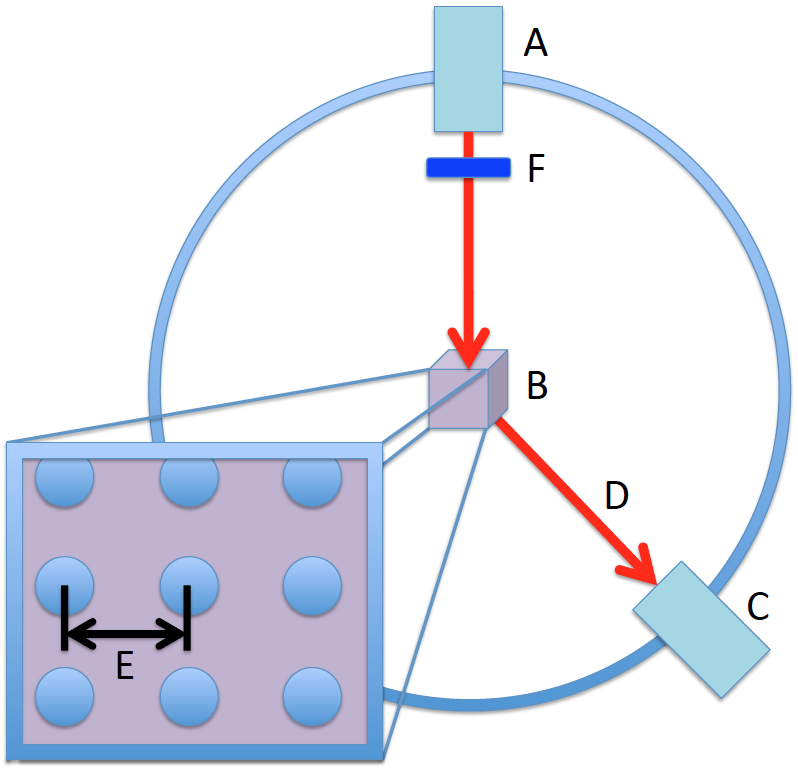
\includegraphics[width=3.in]{appar.png}}
\caption{ \small{A conceptual illustration of the x-ray apparatus and the individual components, also including a portion of the lattice structure. A)\,Copper target x-ray tube\,[x-ray source] B)\,Crystalline sample\,(NaCl/LiF) C)\,Photon detecting Geiger-Muller tube\,[detector] D)\,Source beam E)\,Lattice constant/spacing F)\,Nickel filter \label{appar}}}
  \end{center}
\end{figure}
\clearpage
\section{Procedure and Relevant Equations}


% you always need to end an environment { } you have started--just like in C

Before measurements were conducted on the crystalline samples, backgrounds for each sample were evaluated. Considerable background was generated from scattered x-rays, so the added counts were subtracted from the crystal sample measurements. Estimates of maximum count angles were predetermined, and only certain angle ranges were swept for the background analysis. Isolating the angle in equation\,\ref{lat}, the predicted values for the NaCl K$_\beta$ peaks of n=1 and n=2 were approximately 14.0\degree and 29.0\degree. The NaCl K$_\alpha$ peaks of n=1 and n=2 were about 16.0\degree and 33.0\degree. Predicted values of the LiF K$_\beta$ peaks of n=1 and n=2 were 20.0\degree and 44.0\degree. The LiF K$_\alpha$ peaks of n=1 and n=2 were about 22.0\degree and 49.0\degree.
\\
\indent For NaCl, background angles measured for n=1 were 12.5\degree--17.0\degree, and the n=2 angles were 28.0\degree--34.5\degree. The angles for the LiF background for n=1 and n=2 were 17.0\degree--23.5\degree and 41.5\degree--44.5\degree, respectively. Counts were recorded for 45\,seconds for the NaCl angles, and 180\,seconds for the LiF angles. The LiF sample time interval was significantly longer due to excessive noise background when applying the Ni filter. The exact preceding procedure was replicated while placing the crystal sample of NaCl and LiF in the center of the apparatus for the correlating time intervals. The Ni filter was inserted into the system past the x-ray source to distinguish the K$_\alpha$ and K$_\beta$ lines for analysis.

\begin{equation}
\textnormal{a$_0$}=\frac{\textnormal{n}\lambda}{\sin(\theta)}
\label{lat}
\end{equation}
 
Equation\,\ref{lat} was derived from the Bragg condition, but the lattice constant of the sample, a$_0$, was isolated for computation. The x-ray wavelength, $\lambda$, corresponds to the angle between the emitter and detector, $\theta$, and integer values, n.




\section{Calculation of Results and Errors}
\subsection{Fit Justification}
Peaks generally consisted of three points, therefore instead of fitting a Gaussian relation, lines were fit between every point, and more importantly, the highest points were considered the peaks. 

\subsection{NaCl Sample}

\begin{figure}[h!]
  \begin{center}
\centerline{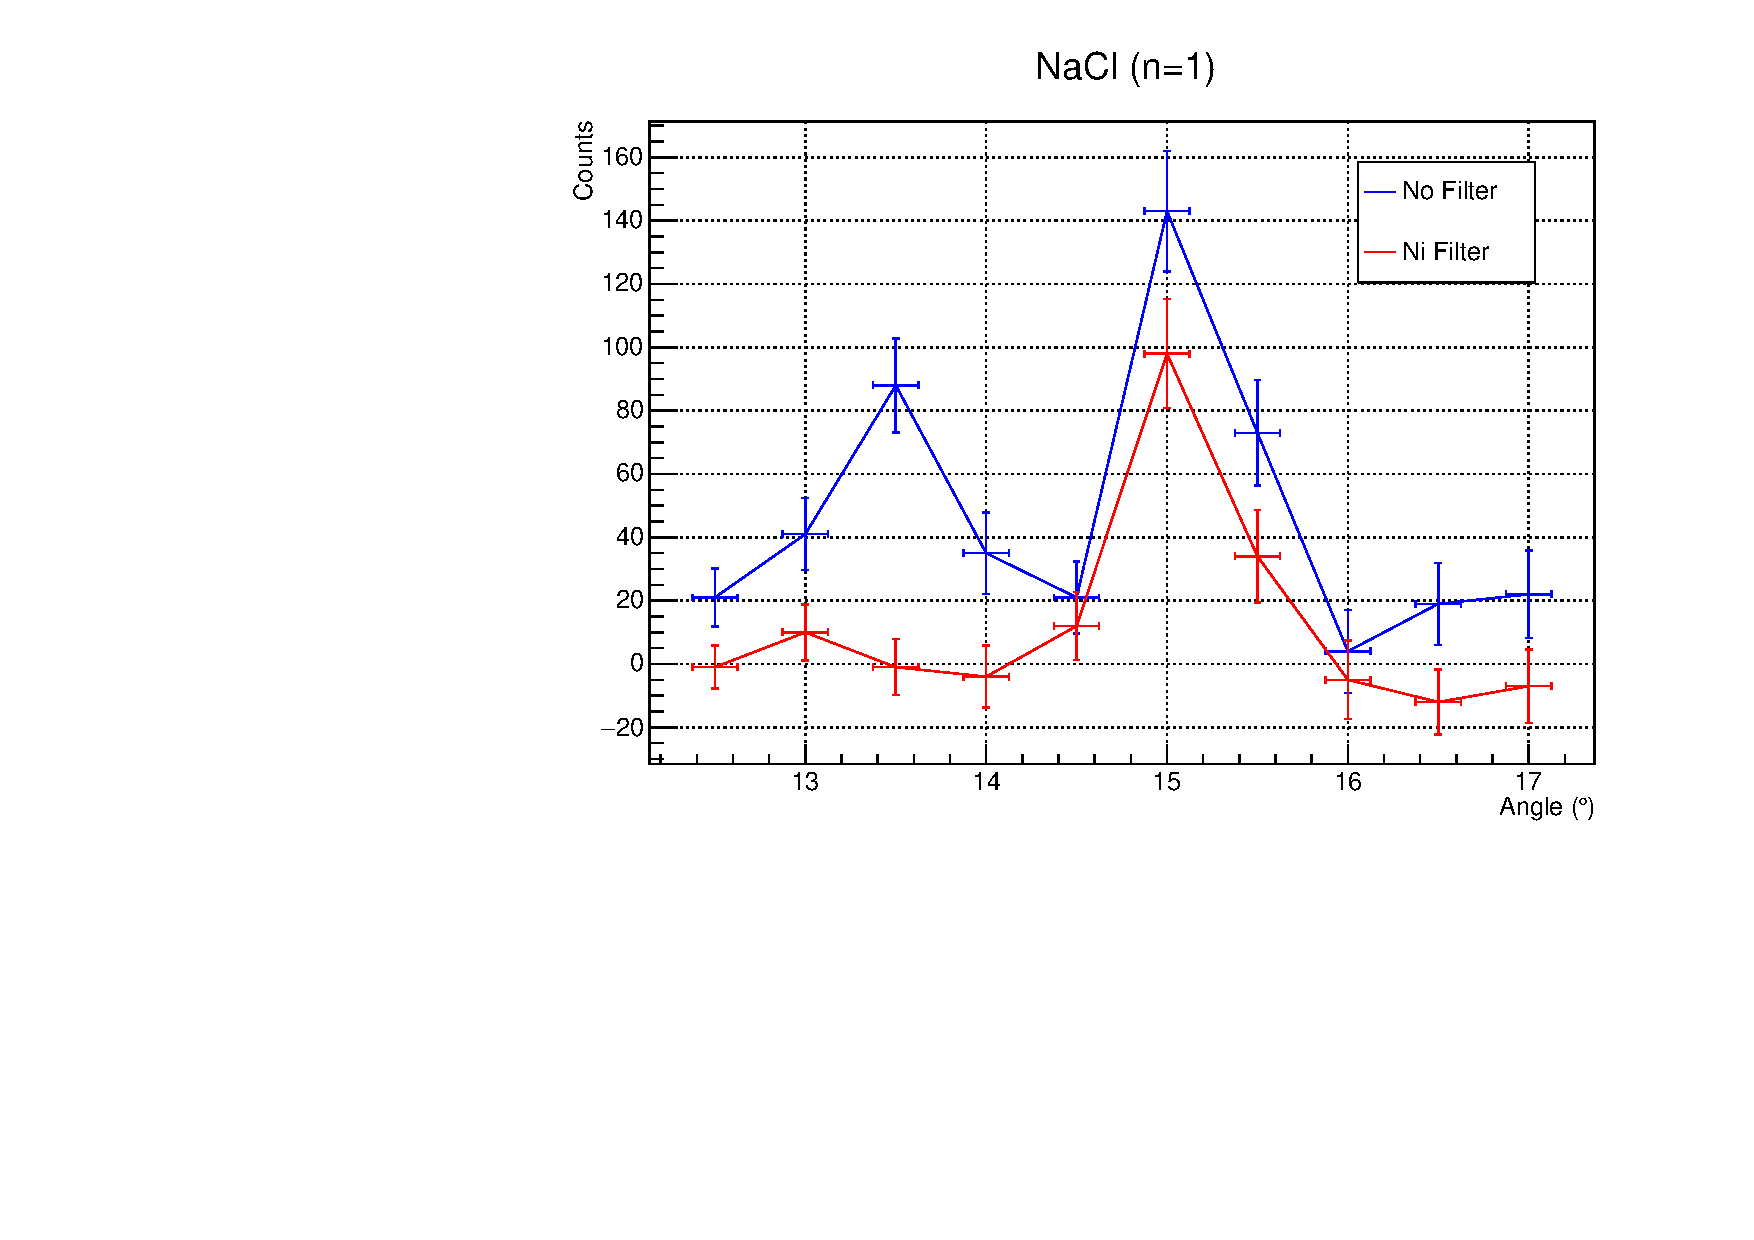
\includegraphics[width=3.5in]{nacl1.pdf}}
\caption{ \small{NaCl maxima peaks for K$_\beta$ and K$_\alpha$ correlating to n=1. The K$_\beta$ peak\,(left peak) is identified due to the extinguished peak when a Ni filter is introduced. \label{nacl1}}}
  \end{center}
\end{figure}

\begin{figure}[h!]
  \begin{center}
\centerline{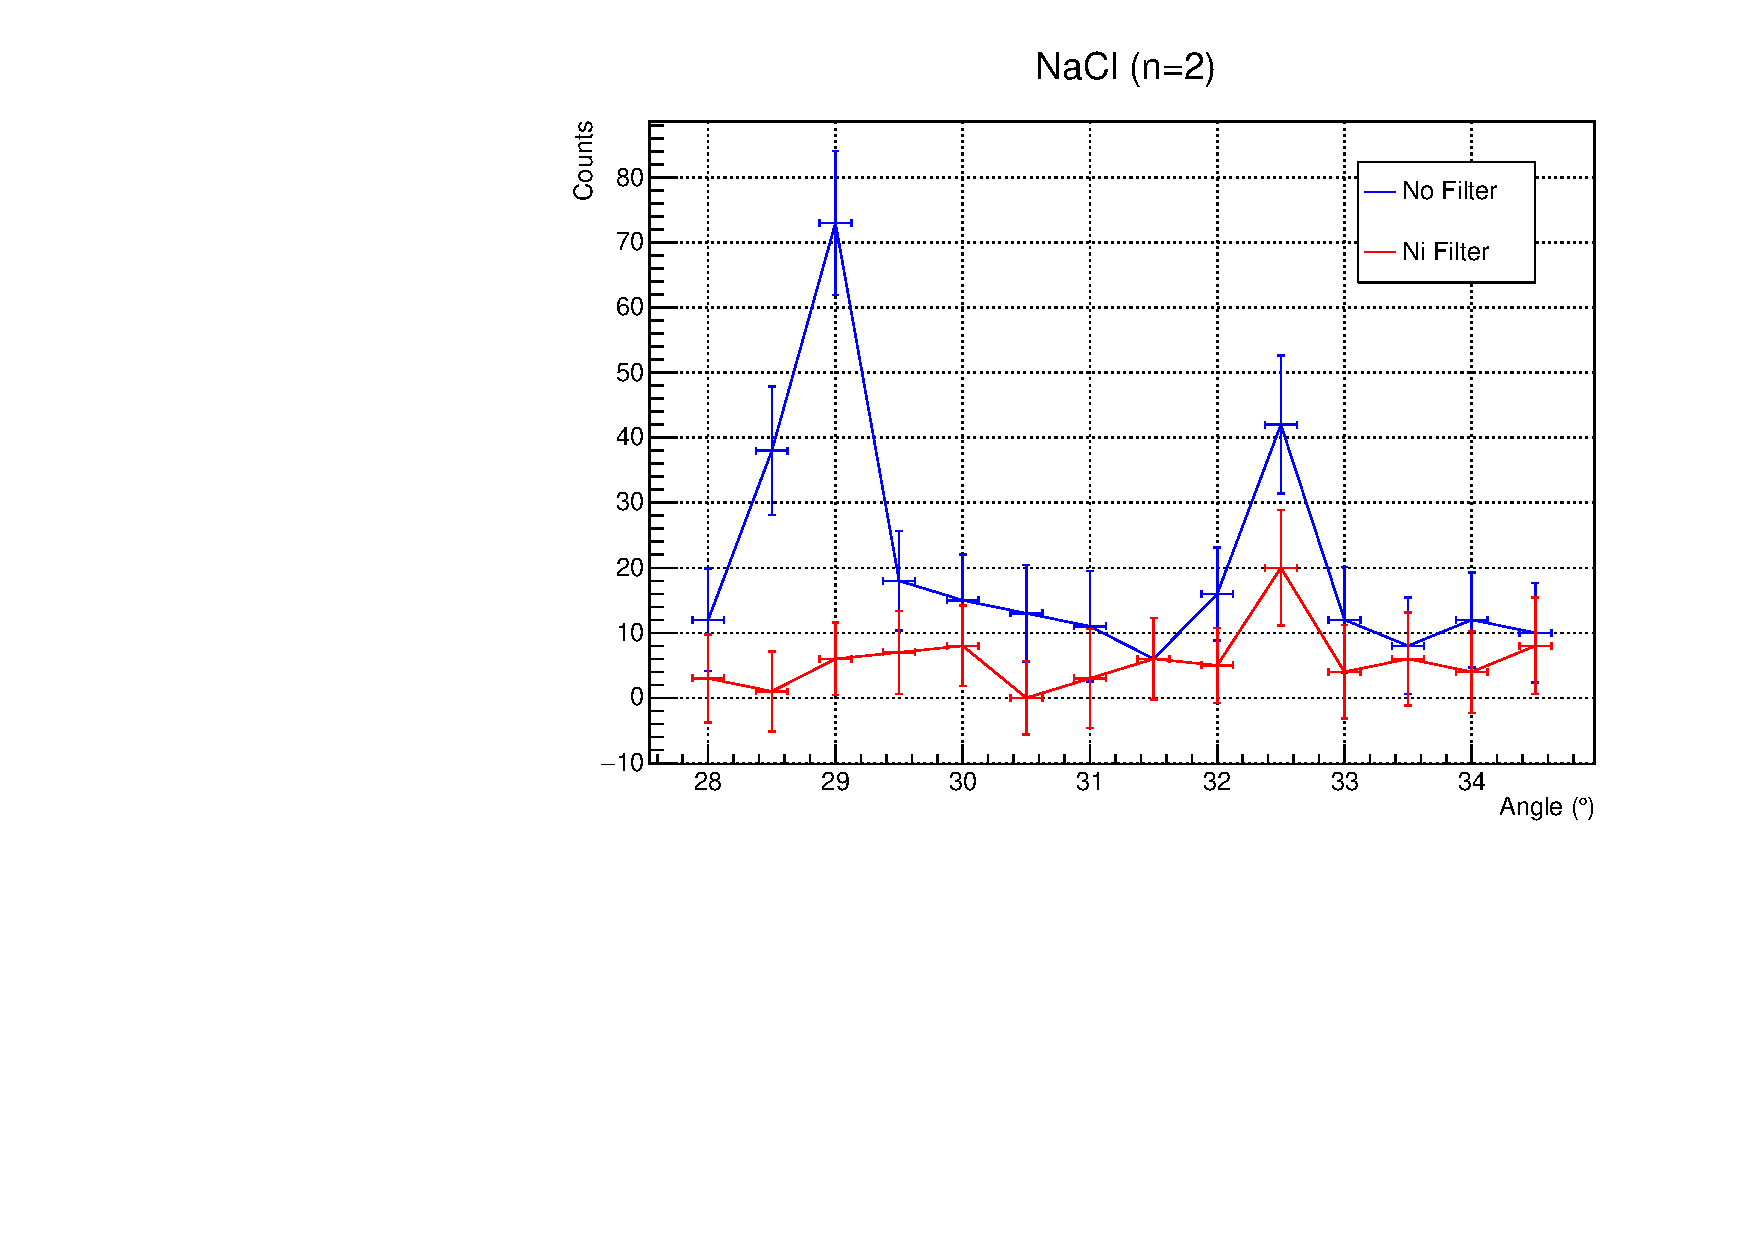
\includegraphics[width=3.5in]{nacl2.pdf}}
\caption{ \small{NaCl maxima peaks for K$_\beta$ and K$_\alpha$ correlating to n=2. The K$_\beta$ peak\,(left peak) is identified due to the extinguished peak when a Ni filter is introduced. \label{nacl2}}}
  \end{center}
\end{figure}

Figure\,\ref{nacl1} yielded the n=1 maximum count peaks at 13.5\degree$\pm$0.3\degree\,for K$_\beta$, and 15.0\degree$\pm$0.3\degree\,for K$_\alpha$. The NaCl n=2 maximum count peaks in figure\,\ref{nacl2} for K$_\beta$ was 29.0\degree$\pm$0.3\degree, and 32.5\degree$\pm$0.3\degree\,for the K$_\alpha$ peak.

\vfill\eject


\subsection{LiF Sample}

\begin{figure}[h!]
  \begin{center}
\centerline{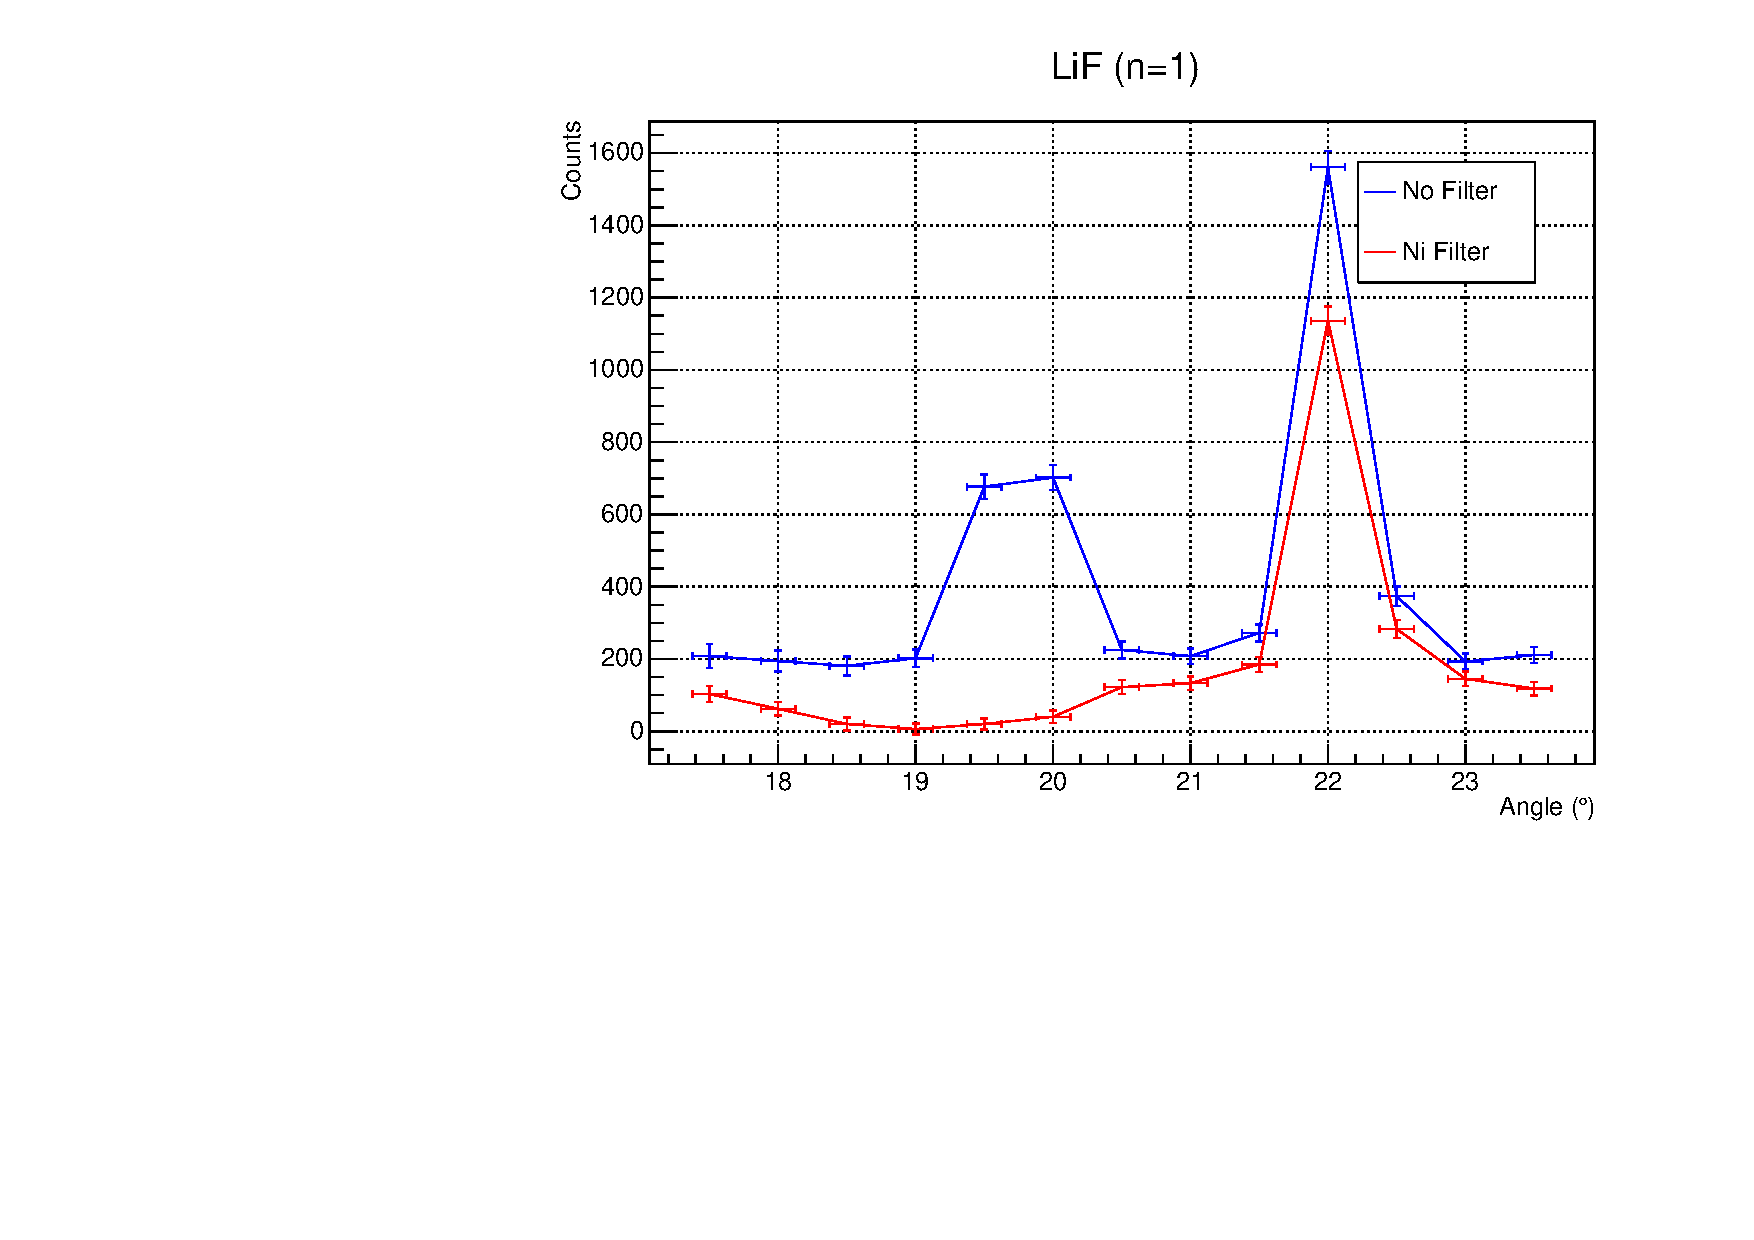
\includegraphics[width=3.5in]{lif1.pdf}}
\caption{ \small{LiF maxima peaks for K$_\beta$ and K$_\alpha$ correlating to n=1. The K$_\beta$ peak\,(left peak) is identified due to the extinguished peak when a Ni filter is introduced. \label{lif1}}}
  \end{center}
\end{figure}

\begin{figure}[h!]
  \begin{center}
\centerline{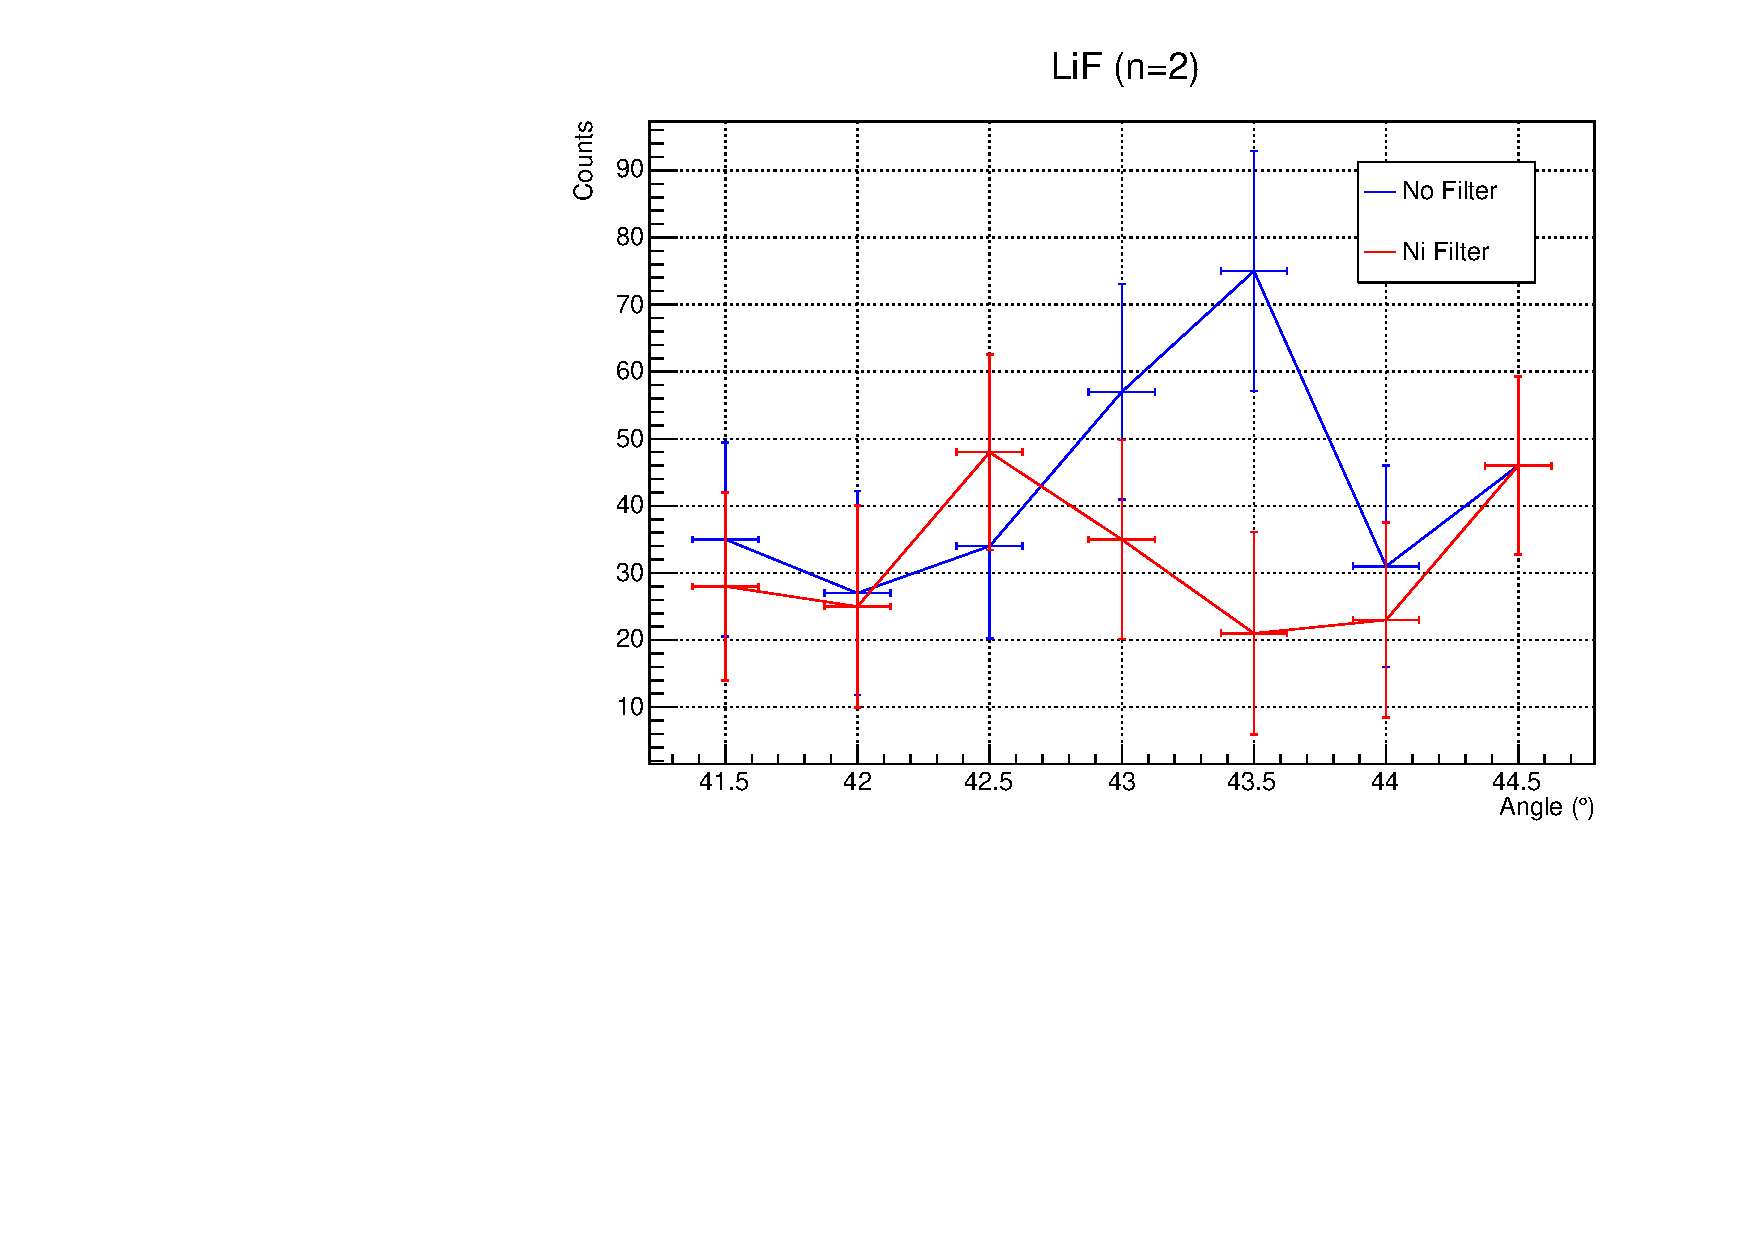
\includegraphics[width=3.5in]{lif2.pdf}}
\caption{ \small{LiF maxima peaks for K$_\beta$ and K$_\alpha$ correlating to n=2. Only the K$_\beta$ peak is present in this plot, which is seen at 43.5\degree. \label{lif2}}}
  \end{center}
\end{figure}

Figure\,\ref{lif1} yielded the n=1 maximum count peaks at 20.0\degree$\pm$0.3\degree\,for K$_\beta$, and 22.0\degree$\pm$0.3\degree\,for K$_\alpha$. The NaCl n=2 maximum count peaks in figure\,\ref{lif2} for K$_\beta$ was 43.5\degree$\pm$0.3\degree. The K$_\alpha$ peak, for n=2, was predetermined to be measured at approximately 50.0\degree, but due to the apparatus angular limitations, this angle wasn't able to be achieved.
\vfill\eject


\subsection{Lattice Constant Results}
 \begin{table}[h!] 
\caption{Experimental lattice constant and literature values of crystal samples of K$_\beta$ peaks}
    %table caption at the top is standard
\label{t1}   % labels are used to refer to this in the text
 \begin{center}   % center the table on the page
    \begin{tabular}{|c|c|c|c|} \hline   % tabular environment 
Crystal  & Experimental & Actual & Error \\
 Sample   & Lattice Constant  & Lattice Constant &  \\
       & (pm)  & (pm) &   \\ \hline \hline \hline
NaCl\,(n=1) & 596.3$\pm$10.8 & 564.0 & 3.0$\sigma$ \\ \hline
NaCl\,(n=2) & 574.3$\pm$4.5 & 564.0 & 2.3$\sigma$ \\ \hline
LiF\,(n=1) & 407.0$\pm$4.9 & 403.0 & 0.8$\sigma$ \\ \hline
LiF\,(n=2) & 404.4$\pm$1.9 & 403.0 & 0.8$\sigma$ \\ \hline
     \end{tabular}
  \end{center}
\end{table}

 \begin{table}[h!] 
\caption{Experimental lattice constant and literature values of crystal samples of K$_\alpha$ peaks}
    %table caption at the top is standard
\label{t2}   % labels are used to refer to this in the text
 \begin{center}   % center the table on the page
    \begin{tabular}{|c|c|c|c|} \hline   % tabular environment 
Crystal  & Experimental & Actual & Error \\
 Sample   & Lattice Constant  & Lattice Constant &  \\
       & (pm)  & (pm) &   \\ \hline \hline \hline
NaCl\,(n=1) & 595.8$\pm$9.7 & 564.0 & 3.3$\sigma$ \\ \hline
NaCl\,(n=2) & 574.0$\pm$3.9 & 564.0 & 1.0$\sigma$ \\ \hline
LiF\,(n=1) & 411.6$\pm$4.4 & 403.0 & 1.9$\sigma$ \\ \hline
LiF\,(n=2) & - & - & - \\ \hline
     \end{tabular}
  \end{center}
\end{table}
\vfill\eject

\section{Discussion and Conclusion}

This study led to experimental lattice constants, which were generated from the peak maxima values, resulting in K$_\beta$ values in table\,\ref{t1} and K$_\alpha$ values in table\,\ref{t2}. The NaCl K$_\beta$ for n=1 and n=2 and K$_\alpha$ peaks for n=1 and n=2 were (596.3$\pm$10.8)\,pm, (574.3$\pm$4.5)\,pm, (595.8$\pm$9.7)\,pm, and (574.0$\pm$3.9)\,pm, respectively. The correlating errors compared to the actual value of 564.0\,pm, in order, were 3.0$\sigma$, 2.3$\sigma$, 3.3$\sigma$, and 1.0$\sigma$. 
\\
\indent The LiF K$_\beta$ for n=1 and n=2 and the K$_\alpha$ peaks for n=1 were (407.0$\pm$4.9)\,pm, (404.4$\pm$1.9)\,pm, (411.6$\pm$4.4)\,pm, respectively. The correlating errors compared to the actual value of 403.0\,pm, in order, were 0.8$\sigma$, 0.8$\sigma$, and 1.9$\sigma$.
\\
\indent Low sigma results showed that the experimental LiF measurements were quite accurate in determining the lattice constant. Conversely, the NaCl sigma errors ranged from 2.3$\sigma$ to 3.3$\sigma$, which showed more deviation.
\\
\indent The n=2 peak for the LiF crystal is not included since the apparatus cannot reach the predetermined angle estimation of 49.0\degree. An amplifier was originally between the pre-amplifier and scaler, in figure\,\ref{scheme}, but was removed. Low HV voltages, below 0.400\,kV, generated excessive pulses and produced too much noise when including the amplifier. Figure\,\ref{lif2} exhibited a small peak-like structure, but the counts are consistent to a ``flat" line, which meant that the no-filter peak was in fact the K$_\beta$ peak. This assumption leads to the conclusion that the statistical errors result mainly from the lack of angle measurements and the Poisson error of the counts.

%\section{Acknowledgments}


% the following \setlength is to force the bibliography to have no
% paragraph indentations.Can use vairous units--cm are used here.
\setlength{\parindent}{0cm}

\begin{thebibliography}{99}  % the trailing 99 controls some obscure format--just use

\bibitem{1} \url{http://www.phys.hawaii.edu/~shige/phys481L/XRay.txt}    % {\em } for emphasis, \textbf{ } for boldface

\bibitem{2} \url{http://www.outreach.phy.cam.ac.uk/camphy/xraydiffraction/xraydiffractionindex.htm}

%\bibitem{3} "Multichannel Analyzer (MCA) Application Software." Nuclear Applications Software|ORTEC Scientific Equipment. ORTEC. Web. 5 Nov. 2015.

%\bibitem{3} \url{http://pdg.lbl.gov/2012/tables/rpp2012-sum-leptons.pdf}




\end{thebibliography}





\end{document}

